% 2008 年北京卷文科第 16 题：三棱锥 P-ABC。
% 来源 PDF：普通高考/2008/2008北京文.pdf，SHA256 9d725e3f7011f50eddddd9bebd62825365c218b08fa0c920ac23b57228f590f9
% 原页：第 1 页（A3 三栏）第 3 栏中部，印刷页 427。
% 重绘依据：P 在顶点，A 在左、B 在右、C 在下方居前；PA、PB、PC、AC、BC 实线，
%   被三棱锥遮住的 AB 画虚线；标注位置按原图。
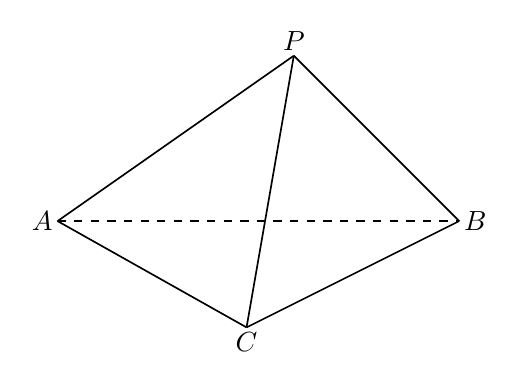
\begin{tikzpicture}[scale=1.5, semithick, every node/.style={inner sep=1.5pt}]
  \coordinate (P) at (0.6,2.6);
  \coordinate (A) at (-1.4,1.2);
  \coordinate (B) at (2.0,1.2);
  \coordinate (C) at (0.2,0.3);
  \draw (P) -- (A);
  \draw (P) -- (B);
  \draw (P) -- (C);
  \draw (A) -- (C);
  \draw (C) -- (B);
  \draw[dashed] (A) -- (B);
  \node[anchor=south] at (P) {$P$};
  \node[anchor=east] at (A) {$A$};
  \node[anchor=west] at (B) {$B$};
  \node[anchor=north] at (C) {$C$};
\end{tikzpicture}
